% Demystifying Agentic AI: Tool Calling, Skills, and Modern Architecture
% Part 1 (motivating examples) and Part 2 (formalization), plus backup slides.
% Compile with: pdflatex agentic_ai_talk.tex   (run twice)
% Red [TODO: ...] tags mark content to replace with captured runs before the talk.

\documentclass[aspectratio=169,14pt]{beamer}
\usetheme[progressbar=none,numbering=none,block=fill]{metropolis}

\usepackage{amsmath,amssymb,mathtools}
\usepackage{tikz,pgfplots}
\usepackage{listings}
\usepackage{array}
\newcolumntype{P}[1]{>{\raggedright\arraybackslash\setlength{\parskip}{0pt}\setlength{\parindent}{0pt}}p{#1}}
\usetikzlibrary{arrows.meta,positioning,calc}
\pgfplotsset{compat=1.16}

% Palette: model action / host observation / highlight. Reuse in Part 2.
\definecolor{actc}{HTML}{1F5FAF}
\definecolor{obsc}{HTML}{B7791F}
\definecolor{hilc}{HTML}{B3261E}
\definecolor{greyc}{HTML}{6B7280}

\newcommand{\task}{\textcolor{greyc}{\textbf{Task}}}
\newcommand{\ask}{\textcolor{actc}{\textbf{Model asks}}}
\newcommand{\ret}{\textcolor{obsc}{\textbf{Host returns}}}
\newcommand{\todo}[1]{\textcolor{hilc}{\footnotesize[TODO: #1]}}
\newcommand{\frownop}{\mathbin{\frown}}

% One row of the run trace: build step, tag, text, decision label.
\newcommand{\trow}[4]{\visible<#1->{#2} & \visible<#1->{#3} & \visible<#1->{\itshape\footnotesize #4} \\[2pt]}

\newcommand{\srow}[4]{\onslide<#1->{\texttt{\scriptsize\textcolor{actc}{#2}}} & \onslide<#1->{\textcolor{obsc}{#3}} & \onslide<#1->{\itshape #4} \\[6pt]}

\definecolor{termbg}{HTML}{1F2933}
\newcommand{\term}[1]{\vspace{-8pt}\begin{center}\begin{tikzpicture}\node[fill=termbg,rounded corners=4pt,inner sep=6pt,text=white,text width=0.93\textwidth,align=left,font=\ttfamily\small] {#1};\end{tikzpicture}\end{center}}
\newcommand{\tdim}[1]{\textcolor{white!55!termbg}{#1}}
\newcommand{\tcall}[1]{\textcolor{cyan!70!white}{#1}}
\newcommand{\tbad}[1]{\textcolor{red!60!white}{#1}}
\newcommand{\tgood}[1]{\textcolor{green!60!white}{#1}}
\newcommand{\shot}[1]{\vfill{\raggedleft\footnotesize\color{greyc} illustrative transcript, real tool output \quad #1/5\par}}
\lstset{basicstyle=\ttfamily\footnotesize,breaklines=true,frame=single,language=Python}

\title{Demystifying Agentic AI}
\subtitle{Tool Calling, Skills, and Modern Architecture}
\author{Kyle Pounder \and Toby Shearman}
\institute{IAB Fall Meeting \\ University of Arizona}
\date{}

\begin{document}

\maketitle

% ---------------------------------------------------------------- Part 1
% C1: the task
\begin{frame}[fragile]{The task}
  \textbf{``The test suite is failing. Fix it.''}
  \vspace{4pt}
  \begin{columns}[T]
    \begin{column}{0.54\textwidth}
      {\footnotesize\color{greyc} What \texttt{run\_tests()} shows (excerpt):}
\begin{lstlisting}[language={},basicstyle=\ttfamily\scriptsize]
    def test_median_even():
>       assert median([4, 1, 3, 2]) == 2.5
E       assert 3 == 2.5
E        +  where 3 = median([4, 1, 3, 2])

FAILED test_stats.py::test_median_even
1 failed, 2 passed in 0.01s
\end{lstlisting}
    \end{column}
    \begin{column}{0.42\textwidth}
      {\footnotesize\color{greyc} The code under test, \texttt{stats.py}:}
\begin{lstlisting}[basicstyle=\ttfamily\scriptsize]
def mean(xs):
    return sum(xs) / len(xs)


def median(xs):
    xs = sorted(xs)
    n = len(xs)
    return xs[n // 2]
\end{lstlisting}
    \end{column}
  \end{columns}
\end{frame}

% Screenshot sequence
\begin{frame}{A coding agent at work}
  \term{
    \tgood{>} The test suite is failing. Fix it.\\[6pt]
    $\bullet$ I'll start by running the tests.\\[3pt]
    \tcall{$\bullet$ run\_tests()}\\
    \tdim{\ \ FAILED test\_stats.py::test\_median\_even}\\
    \tdim{\ \ assert 3 == 2.5 \ \ (median([4, 1, 3, 2]) is 3)}\\
    \tdim{\ \ 1 failed, 2 passed}
  }
  \shot{1}
\end{frame}

\begin{frame}{A coding agent at work}
  \term{
    \tdim{\tgood{$\checkmark$} run\_tests() \ \ 1 failed, 2 passed}\\[6pt]
    $\bullet$ The failure is in median. Let me read it.\\[3pt]
    \tcall{$\bullet$ read\_file("stats.py")}\\
    \tdim{\ \ def median(xs):}\\
    \tdim{\ \ \ \ \ \ xs = sorted(xs)}\\
    \tdim{\ \ \ \ \ \ n = len(xs)}\\
    \tdim{\ \ \ \ \ \ return xs[n // 2]}
  }
  \shot{2}
\end{frame}

\begin{frame}{A coding agent at work}
  \term{
    \tdim{\tgood{$\checkmark$} run\_tests() \ \ 1 failed, 2 passed}\\
    \tdim{\tgood{$\checkmark$} read\_file("stats.py")}\\[6pt]
    $\bullet$ For even lengths it should average the middle two.\\[3pt]
    \tcall{$\bullet$ edit\_file(}\\
    \tcall{\ \ path: "stats.py",}\\
    \tcall{\ \ old\_text: "return xs[n//2]",}\\
    \tcall{\ \ new\_text: "if n \% 2 == 0:}\\
    \tcall{\ \ \ \ \ \ \ \ return (xs[n // 2 - 1] + xs[n // 2]) / 2}\\
    \tcall{\ \ \ \ \ \ \ return xs[n // 2]")}\\
    \tbad{\ \ error: old\_text not found in stats.py}
  }
  \shot{3}
\end{frame}

\begin{frame}{A coding agent at work}
  \term{
    \tdim{\tgood{$\checkmark$} run\_tests() \ \ 1 failed, 2 passed}\\
    \tdim{\tgood{$\checkmark$} read\_file("stats.py")}\\
    \tdim{\tbad{$\times$} edit\_file(...) \ \ error: old\_text not found}\\[6pt]
    $\bullet$ The spacing didn't match. Retrying with the exact text.\\[3pt]
    \tcall{$\bullet$ edit\_file(}\\
    \tcall{\ \ path: "stats.py",}\\
    \tcall{\ \ old\_text: "return xs[n // 2]",}\\
    \tcall{\ \ new\_text: "if n \% 2 == 0: ... return xs[n // 2]")}\\
    \tdim{\ \ ok}
  }
  \shot{4}
\end{frame}

\begin{frame}{A coding agent at work}
  \term{
    \tdim{\tgood{$\checkmark$} run\_tests() \ \ 1 failed, 2 passed}\\
    \tdim{\tgood{$\checkmark$} read\_file("stats.py")}\\
    \tdim{\tbad{$\times$} edit\_file(...) \ \ error: old\_text not found}\\
    \tdim{\tgood{$\checkmark$} edit\_file(...) \ \ ok}\\[6pt]
    \tcall{$\bullet$ run\_tests()}\\
    \tdim{\ \ 3 passed}\\[6pt]
    $\bullet$ Fixed: median now averages the two middle values for even-length lists. All 3 tests pass.
  }
  \shot{5}
\end{frame}

% Reveal: three players
\begin{frame}{That looks like magic. What is going on?}
  \centering
  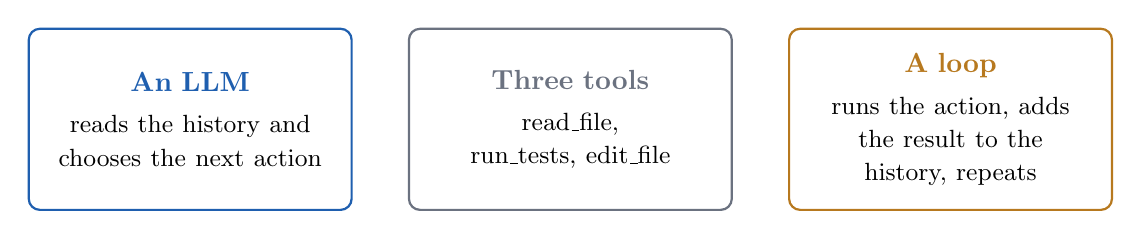
\begin{tikzpicture}[
      box/.style={draw,rounded corners,thick,minimum width=4.1cm,minimum height=2.3cm,align=center,text width=3.7cm},
      >=Stealth]
    \node[box,draw=actc] (m) {\textbf{\textcolor{actc}{An LLM}}\\[3pt]\small reads the history and chooses the next action};
    \node[box,draw=greyc,right=0.7cm of m] (t) {\textbf{\textcolor{greyc}{Three tools}}\\[3pt]\small read\_file, run\_tests, edit\_file};
    \node[box,draw=obsc,right=0.7cm of t] (l) {\textbf{\textcolor{obsc}{A loop}}\\[3pt]\small runs the action, adds the result to the history, repeats};
  \end{tikzpicture}

  \vspace{14pt}
  Next: each piece, with the math that pins it down.
\end{frame}

% ---------------------------------------------------------------- Part 2
\begin{frame}{What is a tool?}
  \[
    \tau = (\text{name},\, S,\, f), \qquad S \subseteq \mathcal{X}, \qquad f : S \to \mathcal{Y}
  \]
  \small
  Our example, $\tau = \texttt{edit\_file}$:\\[4pt]
  \begin{tabular}{@{}l P{10.6cm}@{}}
    $\mathcal{X}$ & all argument objects: key--value pairs of strings (JSON) \\[3pt]
    $S$ & objects with exactly the keys \texttt{path}, \texttt{old\_text}, \texttt{new\_text} \\[3pt]
    $f$ & replace \texttt{old\_text} by \texttt{new\_text} in the file; return ``ok'' or an error message \\[3pt]
    $\mathcal{Y}$ & text \\
  \end{tabular}
  \vfill
  The model sees $(\text{name}, S)$ and writes down a call. The host holds $f$: it checks $x \in S$, then runs $f$. If $x \notin S$, it returns an error message instead.
\end{frame}

\begin{frame}{Tools in the example}
  \small
  \begin{tabular}{@{}l P{3.6cm} P{3.4cm} P{3.4cm}@{}}
    \textbf{name} & \textbf{$S$: allowed arguments} & \textbf{$f$: what the host does} & \textbf{result in $\mathcal{Y}$} \\ \hline
    \rule{0pt}{12pt}\texttt{read\_file} & a path (string) & reads the file & its text \\[3pt]
    \texttt{run\_tests} & none, or a path & runs the test suite & pass/fail summary, traceback \\[3pt]
    \texttt{edit\_file} & a path, the old text, the new text & replaces old with new & ``ok'' or an error message \\
  \end{tabular}
  \vfill
  $S$ checks only the \emph{shape} of the arguments. Whether \texttt{old\_text} occurs in the file is checked when $f$ runs, and a failure comes back as an ordinary result in $\mathcal{Y}$. $T=\{\tau_1,\dots,\tau_k\}$ denotes the agent's set of tools.
\end{frame}

\begin{frame}{What the LLM sees and can do}
  \small
  \textbf{Sees} a history $h_t \in H$: the user's request, then one (action, result) pair per step so far.
  \footnotesize
  \[
    \begin{aligned}
      h_2 = \Big( & \text{``The test suite is failing. Fix it.''}, \\
      & \big(\textcolor{actc}{\texttt{call(run\_tests, \{\})}},\ \textcolor{obsc}{\text{``1 failed, 2 passed''}}\big), \\
      & \big(\textcolor{actc}{\texttt{call(read\_file, \{path: "stats.py"\})}},\ \textcolor{obsc}{\text{``def median(xs): \ldots''}}\big) \Big)
    \end{aligned}
  \]
  \small
  \textbf{Can choose} an action $a_t \in A = \{\text{answer}(m)\} \cup \{\text{call}(\tau, x) : \tau \in T,\ x \in \mathcal{X}\}$:
  \vspace{4pt}

  \footnotesize
  \begin{tabular}{@{}l l@{}}
    \textcolor{actc}{\texttt{call(edit\_file, \{path: "stats.py", \ldots\})}} & run a tool $\tau$ on arguments $x$ \\[2pt]
    \textcolor{actc}{\texttt{call(run\_tests, \{\})}} & run a tool $\tau$ on arguments $x$ \\[2pt]
    \textcolor{actc}{\texttt{answer("Fixed median; 3 tests pass.")}} & reply to the user with text $m$, and stop \\
  \end{tabular}
  \vfill
  {\color{greyc} $H$ is the set of all such histories; $x$ can be any argument object in $\mathcal{X}$.}
\end{frame}

\begin{frame}{The LLM chooses}
  \[
    \pi : H \to \Delta(A), \qquad a_t \sim \pi(\cdot \mid h_t)
  \]
  \small
  $\Delta(A)$ is the set of probability distributions over $A$. Given the history, the LLM puts a probability on every possible next action, and one is drawn at random ($\sim$).\\[8pt]
  \centering
  {\footnotesize $\pi(\cdot \mid h_2)$ for our example \color{greyc}(made-up numbers)}\\[4pt]
  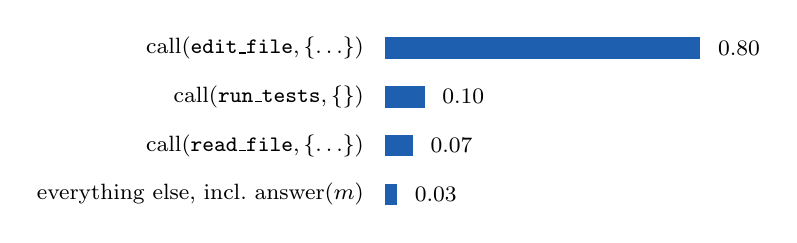
\begin{tikzpicture}[x=1cm,y=-0.62cm]
    \foreach \i/\lab/\pr in {0/{$\text{call}(\texttt{edit\_file},\{\ldots\})$}/0.80, 1/{$\text{call}(\texttt{run\_tests},\{\})$}/0.10, 2/{$\text{call}(\texttt{read\_file},\{\ldots\})$}/0.07, 3/{everything else, incl.\ $\text{answer}(m)$}/0.03} {
      \node[anchor=east,font=\footnotesize] at (0,\i) {\lab};
      \fill[actc] (0.15,\i-0.22) rectangle ({0.15+5*\pr},\i+0.22);
      \node[anchor=west,font=\footnotesize] at ({0.25+5*\pr},\i) {\pr};
    }
  \end{tikzpicture}
  \vfill
  \raggedright\footnotesize\color{greyc}
  How $\pi$ learns to choose well comes from training; for this talk it is a black box we sample from.
\end{frame}

\begin{frame}{The loop}
  \small
  \[
    o(\tau, x) = \begin{cases} f_\tau(x) & x \in S_\tau \\ \text{an error message} & \text{otherwise} \end{cases}
  \]
  \[
    h_{t+1} = h_t \frownop \big(a_t,\ o(\tau, x)\big) \ \text{ if } a_t = \text{call}(\tau, x)
  \]
  \[
    \text{stop when } a_t = \text{answer}(m) \ \text{ or } \ t = N
  \]
  \centering
  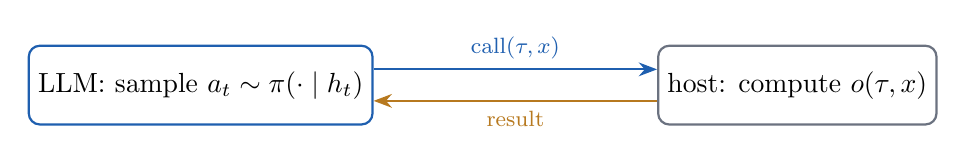
\begin{tikzpicture}[
      box/.style={draw,rounded corners,thick,minimum width=3.4cm,minimum height=1cm,align=center},
      >=Stealth]
    \node[box,draw=actc] (m) {LLM: sample $a_t \sim \pi(\cdot\mid h_t)$};
    \node[box,draw=greyc,right=3.6cm of m] (h) {host: compute $o(\tau,x)$};
    \draw[->,thick,actc] ([yshift=0.2cm]m.east) -- node[above,font=\footnotesize] {$\text{call}(\tau,x)$} ([yshift=0.2cm]h.west);
    \draw[->,thick,obsc] ([yshift=-0.2cm]h.west) -- node[below,font=\footnotesize] {result} ([yshift=-0.2cm]m.east);
  \end{tikzpicture}
  \vfill
  \raggedright\footnotesize
  $\frownop$ appends one entry to the end of the history. $h_0$ is the user's request. $N$ is a step budget.
\end{frame}

\begin{frame}{The loop, on our example}
  \small
  $h_0$ = ``The test suite is failing. Fix it.'' Each step appends one (action, result) pair.\\[6pt]
  \footnotesize
  \setlength{\tabcolsep}{4pt}\begin{tabular}{@{}c l l@{}}
    $t$ & \textcolor{actc}{action $a_t$} & \textcolor{obsc}{result $o(\tau,x)$} \\ \hline
    \rule{0pt}{11pt}0 & \texttt{call(run\_tests, \{\})} & 1 failed, 2 passed \\[2pt]
    1 & \texttt{call(read\_file, \{path: "stats.py"\})} & the source of \texttt{stats.py} \\[2pt]
    2 & \texttt{call(edit\_file, \{old\_text: "return xs[n//2]", \ldots\})} & \textcolor{hilc}{error: old\_text not found} \\[2pt]
    3 & \texttt{call(edit\_file, \{old\_text: "return xs[n // 2]", \ldots\})} & ok \\[2pt]
    4 & \texttt{call(run\_tests, \{\})} & 3 passed \\[2pt]
    5 & \texttt{answer("Fixed median; 3 tests pass.")} & (loop stops) \\
  \end{tabular}
\end{frame}

% ---------------------------------------------------------------- Part 3
\begin{frame}{Be the policy (2.5 min)}
  \begin{columns}[T]
    \begin{column}{0.58\textwidth}
      \footnotesize The history $h_2$ for a new bug:\\[3pt]
      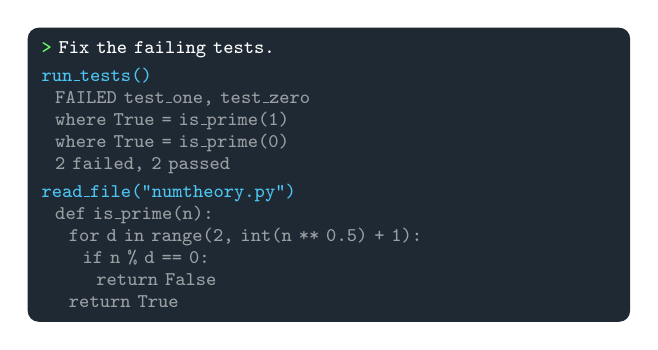
\begin{tikzpicture}
        \node[fill=termbg,rounded corners=4pt,inner sep=5pt,text=white,text width=7.3cm,align=left,font=\ttfamily\scriptsize] {
          \tgood{>} Fix the failing tests.\\[2pt]
          \tcall{run\_tests()}\\
          \tdim{\ \ FAILED test\_one, test\_zero}\\
          \tdim{\ \ where True = is\_prime(1)}\\
          \tdim{\ \ where True = is\_prime(0)}\\
          \tdim{\ \ 2 failed, 2 passed}\\[2pt]
          \tcall{read\_file("numtheory.py")}\\
          \tdim{\ \ def is\_prime(n):}\\
          \tdim{\ \ \ \ for d in range(2, int(n ** 0.5) + 1):}\\
          \tdim{\ \ \ \ \ \ if n \% d == 0:}\\
          \tdim{\ \ \ \ \ \ \ \ return False}\\
          \tdim{\ \ \ \ return True}
        };
      \end{tikzpicture}
    \end{column}
    \begin{column}{0.40\textwidth}
      \footnotesize \textbf{What should $a_2$ be? Vote.}\\[3pt]
      \begin{tabular}{@{}l P{3.8cm}@{}}
        (a) & \texttt{\scriptsize call(run\_tests, \{\})}\\
        \multicolumn{2}{@{}l@{}}{\uncover<2->{\color{greyc}\quad repeats what we know; wastes a step}}\\[1pt]
        (b) & \texttt{\scriptsize call(edit\_file, \{path: "numtheory.py", \ldots\})}\\
        \multicolumn{2}{@{}l@{}}{\uncover<2->{\color{greyc}\quad reasonable: adds the missing $n<2$ case}}\\[1pt]
        (c) & \texttt{\scriptsize call(edit\_file, \{path: "test\_numtheory.py", \ldots\})}\\
        \multicolumn{2}{@{}l@{}}{\uncover<2->{\color{hilc}\quad passes without fixing the code}}\\[1pt]
        (d) & \texttt{\scriptsize answer("The tests are wrong.")}\\
        \multicolumn{2}{@{}l@{}}{\uncover<2->{\color{greyc}\quad not supported by the history}}\\
      \end{tabular}
    \end{column}
  \end{columns}
  \vspace{2pt}
  \uncover<2->{\footnotesize The room's votes are an estimate of $\pi(\cdot \mid h_2)$.}
\end{frame}

\begin{frame}{Be the host (2.5 min)}
  \footnotesize
  You are the host. The tool is $\tau = \texttt{edit\_file}$, with $S$ = objects with keys \texttt{path}, \texttt{old\_text}, \texttt{new\_text}, all strings. The file is \texttt{numtheory.py} from the last slide. For each call, what is $o(\tau, x)$?\\[8pt]
  \setlength{\tabcolsep}{4pt}
  \begin{tabular}{@{}c l l@{}}
    & \textbf{call} & \onslide<2->{\textbf{$o(\tau,x)$}} \\ \hline
    \rule{0pt}{11pt}1 & \parbox[t]{7.6cm}{\texttt{\scriptsize old\_text: "for d in range(2, int(n ** 0.5) + 1):",\\ new\_text: "\ldots"}} & \onslide<2->{\texttt{\scriptsize ok}} \\[7pt]
    2 & \parbox[t]{7.6cm}{\texttt{\scriptsize old\_text: "for d in range(2, int(n**0.5) + 1):",\\ new\_text: "\ldots"}} & \onslide<2->{\parbox[t]{4.6cm}{\textcolor{hilc}{\texttt{\scriptsize error: old\_text not found in numtheory.py}}}} \\[7pt]
    3 & \parbox[t]{7.6cm}{\texttt{\scriptsize old\_text: "return True"}\\ {\scriptsize (no \texttt{new\_text} key)}} & \onslide<2->{\parbox[t]{4.6cm}{\textcolor{hilc}{\texttt{\scriptsize error: invalid arguments for edit\_file (expected keys: path, old\_text, new\_text)}}}} \\[7pt]
    4 & \parbox[t]{7.6cm}{\texttt{\scriptsize old\_text: "return",\\ new\_text: "yield"}} & \onslide<2->{\parbox[t]{4.6cm}{\textcolor{hilc}{\texttt{\scriptsize error: old\_text occurs 2 times in numtheory.py}}}} \\
  \end{tabular}
  \vfill
  {\color{greyc} In every call, path is "numtheory.py".}
\end{frame}

\begin{frame}{Debrief (1 min)}
  \begin{enumerate}
    \item Where did the \emph{choosing} happen, and where did the \emph{checking} happen?\\
      {\small\color{greyc} the policy $\pi$ versus the schema $S$ and the function $f$}
    \item Call 3 was rejected before $f$ ran. Why is it still useful that the model sees that error?\\
      {\small\color{greyc} errors are observations, so the loop can recover}
    \item If \texttt{edit\_file} could also delete files, what would you change?\\
      {\small\color{greyc} a scoped tool set $T_t \subseteq T$}
  \end{enumerate}
\end{frame}

% ---------------------------------------------------------------- Part 4
\begin{frame}[fragile]{What is a skill?}
  \begin{columns}[T]
    \begin{column}{0.38\textwidth}
      \small A folder of instructions, plus optional scripts. It runs nothing by itself.
\begin{lstlisting}[language={},basicstyle=\ttfamily\scriptsize,frame=none]
fix-failing-tests/
  SKILL.md
\end{lstlisting}
    \end{column}
    \begin{column}{0.60\textwidth}
\begin{lstlisting}[language={},basicstyle=\ttfamily\scriptsize]
---
name: fix-failing-tests
description: Use when asked to fix
  failing tests or a failing build.
---
1. Run the full test suite first; read
   the failure before opening any file.
2. Read the code under test, not just
   the test.
3. Make the smallest change that fixes
   the failure.
4. Do not edit a test to make it pass
   unless asked.
5. Rerun the full suite, not just the
   failing test.
6. Report what you changed and why.
\end{lstlisting}
    \end{column}
  \end{columns}
\end{frame}

\begin{frame}{How the agent uses a skill}
  \begin{itemize}
    \item<1-> \textbf{Session start:} the agent sees only each skill's name and one-line description.
    \item<2-> \textbf{A task arrives} (``fix the failing tests''): the description matches, so the agent reads \texttt{SKILL.md} with an ordinary file-read call.
    \item<2-> \textbf{Now} the instructions are in its context. It may also run the bundled script, another ordinary tool call.
  \end{itemize}
  \vfill
  \uncover<2->{\begin{block}{}
    A tool is something the agent can \emph{do}. A skill is something it \emph{knows how to do well}.
  \end{block}}
\end{frame}

\begin{frame}{Why load on demand}
  \small
  \textbf{Context budget.} $n$ skills, each with a description of $d$ tokens and instructions of $c$ tokens; $k$ skills used:
  \[
    \underbrace{n(d+c)}_{\text{load everything}} \quad\text{vs.}\quad \underbrace{nd + kc}_{\text{index, then load on demand}}
  \]
  Illustrative numbers: $n=50$, $d=50$, $c=2000$, $k=1$ gives $102{,}500$ versus $4{,}500$ tokens.

  \vspace{6pt}
  \textbf{Loading a skill is a tool call.} It changes what the model conditions on, not the model itself:
  \[
    h_{t+1} = h_t \frownop \big(\text{call}(\text{read\_file}, \texttt{SKILL.md}),\ \text{text of SKILL.md}\big)
  \]
  \textbf{Scoping.} At each step the agent sees only $T_t \subseteq T$: fewer ways to be wrong, and least privilege.
\end{frame}

% ---------------------------------------------------------------- Part 5
\begin{frame}{MCP: one protocol instead of $N\cdot M$ integrations}
  \centering
  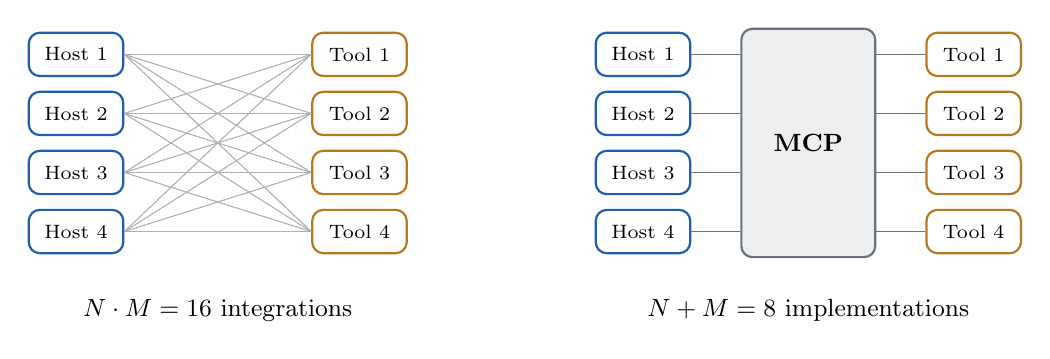
\begin{tikzpicture}[
      host/.style={draw=actc,thick,rounded corners,minimum width=1.2cm,minimum height=0.55cm,font=\scriptsize},
      tool/.style={draw=obsc,thick,rounded corners,minimum width=1.2cm,minimum height=0.55cm,font=\scriptsize},
      hub/.style={draw=greyc,thick,fill=greyc!12,rounded corners,minimum width=1.7cm,minimum height=2.9cm,font=\bfseries\small},
    ]
    \foreach \i in {1,2,3,4} {
      \node[host] (lh\i) at (0,{-0.75*\i}) {Host \i};
      \node[tool] (lt\i) at (3.6,{-0.75*\i}) {Tool \i};
      \node[host] (rh\i) at (7.2,{-0.75*\i}) {Host \i};
      \node[tool] (rt\i) at (11.4,{-0.75*\i}) {Tool \i};
    }
    \foreach \i in {1,2,3,4} {
      \foreach \j in {1,2,3,4} {
        \draw[greyc!55] (lh\i.east) -- (lt\j.west);
      }
    }
    \node[hub] (hub) at (9.3,-1.875) {MCP};
    \foreach \i in {1,2,3,4} {
      \draw[greyc] (rh\i.east) -- (rh\i.east -| hub.west);
      \draw[greyc] (rt\i.west) -- (rt\i.west -| hub.east);
    }
    \node[font=\small] at (1.8,-4.0) {$N\cdot M = 16$ integrations};
    \node[font=\small] at (9.3,-4.0) {$N+M = 8$ implementations};
  \end{tikzpicture}

  \vspace{6pt}
  {\small Each AI application implements one side of a shared protocol once, and each tool implements the other side once. For $N=5$ and $M=8$: $40 \to 13$.}
\end{frame}

% ---------------------------------------------------------------- Wrap-up
\begin{frame}{Takeaways}
  \begin{enumerate}
    \item An agent is a model in a loop: it emits structured calls, the host validates and runs them, and the results go back into the history.
    \item Reliability is a design problem: precise schemas, small scoped tool sets, and verification steps (like rerunning the tests) make errors easier to catch.
    \item Skills and MCP are architecture, not magic: skills load know-how on demand, and a shared protocol turns $N\cdot M$ integrations into $N+M$.
  \end{enumerate}
\end{frame}

\begin{frame}[standout]
  Questions?\\[14pt]
  {\footnotesize [TODO: add links (MCP specification, exercise handout) and contact info]}
\end{frame}

% ---------------------------------------------------------------- Backup
\appendix

\begin{frame}[fragile]{Backup: the median bug and its fix}
  \begin{columns}[T]
    \begin{column}{0.48\textwidth}
      {\footnotesize\color{greyc} before}
\begin{lstlisting}[basicstyle=\ttfamily\scriptsize]
def median(xs):
    xs = sorted(xs)
    n = len(xs)
    return xs[n // 2]
\end{lstlisting}
    \end{column}
    \begin{column}{0.48\textwidth}
      {\footnotesize\color{greyc} after}
\begin{lstlisting}[basicstyle=\ttfamily\scriptsize]
def median(xs):
    xs = sorted(xs)
    n = len(xs)
    if n % 2 == 0:
        return (xs[n // 2 - 1]
                + xs[n // 2]) / 2
    return xs[n // 2]
\end{lstlisting}
    \end{column}
  \end{columns}
\end{frame}

\begin{frame}[fragile]{Backup: exercise answer key}
  Fix: add the $n<2$ case. All 4 tests pass afterward.
\begin{lstlisting}[basicstyle=\ttfamily\footnotesize]
def is_prime(n):
    if n < 2:
        return False
    for d in range(2, int(n ** 0.5) + 1):
        if n % d == 0:
            return False
    return True
\end{lstlisting}
\end{frame}

\end{document}
